\documentclass[11pt,a4paper]{article}

\usepackage{graphicx}
\usepackage{xcolor}
\usepackage{geometry}
\usepackage{amsmath}
\usepackage{booktabs}
\usepackage{enumitem}
\usepackage{tabularx}
\usepackage{adjustbox}
\usepackage{fancyhdr}
\usepackage{caption}
\usepackage{etoolbox}
\usepackage[numbers,sort&compress]{natbib}
\bibliographystyle{unsrtnat}
% ragged-right bibliography: avoids justification under/overfull boxes with long DOIs/URLs
\apptocmd{\thebibliography}{\raggedright\footnotesize}{}{}
\setlength{\emergencystretch}{2em}

% hyperref last among content packages
\usepackage[
    colorlinks=true,
    linkcolor=blue!50!black,
    citecolor=blue!40!black,
    urlcolor=blue!50!black,
    bookmarks=true,
    bookmarksnumbered=true,
    unicode=true
]{hyperref}

\geometry{a4paper, top=2.5cm, bottom=2.5cm, left=2.5cm, right=2.5cm}
\setlength{\headheight}{14pt}
\widowpenalty=10000
\clubpenalty=10000

\pagestyle{fancy}
\fancyhf{}
\fancyhead[L]{\small\itshape Forest loss pressure on Indigenous Lands with uncontacted peoples}
\fancyhead[R]{\small\thepage}
\renewcommand{\headrulewidth}{0.3pt}

\captionsetup{font=small, labelfont=bf}

\newcommand{\tipi}{TIPI}

\hypersetup{
    pdftitle={Forest Loss Pressure on Indigenous Lands with Uncontacted Peoples in the Brazilian Amazon (2000-2023)},
    pdfauthor={Mohd Shadab},
    pdfsubject={Open-data geospatial assessment of forest cover change on Indigenous Lands hosting uncontacted peoples},
    pdfkeywords={uncontacted peoples, isolated peoples, Indigenous Lands, deforestation, Brazilian Amazon, Global Forest Change}
}

\begin{document}

\begin{center}
    {\LARGE\bfseries Forest Loss Pressure on Indigenous Lands with Uncontacted Peoples in the Brazilian Amazon: An Open-Data Geospatial Assessment (2000--2023)}\\[10pt]
    {\normalsize Mohd Shadab\thanks{Independent researcher. Correspondence: author's repository (see Data and Code Availability).}}\\[6pt]
    {\small Preprint --- November 2026}
\end{center}

\vspace{6pt}
\begin{center}
\begin{minipage}{0.88\textwidth}
\small
\textbf{Abstract.}
Brazil hosts the world's largest concentration of uncontacted (isolated) Indigenous peoples, yet no published quantitative assessment measures how much forest loss occurs inside and around the Indigenous Lands that host them, as distinct from Indigenous lands in general. Using only open data --- official FUNAI territory boundaries (657 lands), mapped isolated-peoples occupation areas and records from the OPI observatory (115 records; 29 state-confirmed), and the Hansen/UMD Global Forest Change dataset (2000--2023, canopy cover $>$30\%) --- we compare forest loss inside 81 Indigenous Lands with isolated-peoples presence (\tipi{}) against (i) 155 matched non-isolated Indigenous Lands and (ii) surrounding 0--10\,km and 10--50\,km buffer rings. Median loss of year-2000 tree cover inside \tipi{} was 1.01\%, versus 3.66\% in the 0--10\,km ring and 5.30\% in the 10--50\,km ring (Wilcoxon signed-rank $p<10^{-10}$, large effects); \tipi{} also lost significantly less forest than matched controls (2.51\% median; Mann--Whitney $p<10^{-4}$). Pressure is strongly spatially concentrated (Gini 0.63): the ten highest-pressure territories account for nearly half (48.5\%) of aggregate surrounding loss, led by Uru-Eu-Wau-Wau (222{,}349\,ha of ring loss; 35.1\% ring loss share while holding inside loss to 2.27\%) and Ba\'u (153{,}702\,ha ring loss; 23.5\% ring loss share with only 0.25\% inside loss). Ring pressure was strongly associated with distance to urban centers ($\rho=-0.457$, $p<10^{-4}$), reflecting diffuse settlement frontier dynamics. These results quantify, for the first time at territory level, the buffering function of uncontacted peoples' lands and identify where Brazil's protection apparatus --- audited in 2024 as under-staffed and leaving 12 records without any territorial protection --- is most urgently needed. All code, data provenance, and statistics are fully reproducible from the open repository. The study involves no field contact and publishes no settlement locations, in line with the no-contact policy for isolated peoples.
\vspace{4pt}

\textbf{Keywords:} uncontacted peoples; isolated peoples; \textit{povos ind\'igenas isolados}; Indigenous Lands; deforestation; Brazilian Amazon; forest cover change; protected areas; geospatial analysis
\end{minipage}
\end{center}

\section{Introduction}\label{sec:intro}

Uncontacted peoples --- in Brazil's official terminology, \emph{povos ind\'igenas isolados} --- are indigenous groups who maintain no sustained relations with the surrounding national society \citep{pringle2014,survival2025}. Brazil holds the world's largest number of such peoples: FUNAI, the National Foundation of Indigenous Peoples, maintained 114 official records of isolated peoples in 2024, of which the state had confirmed 29 and left twelve without any territorial protection instrument whatsoever \citep{funai_audit_2024}; a 2025 global survey estimates 124 groups in Brazil alone, roughly two-thirds of the world's 196 \citep{survival2025}. For these peoples, forest loss is not only an environmental problem: they depend entirely on the forest for food, medicine, and material culture, they have no acquired immunity to epidemic disease, and their isolation is itself a survival strategy --- formally protected since 1987 by FUNAI's no-contact policy \citep{pringle2014}. The epidemiological record underlines what is at stake: across 117 recorded contact-related epidemics in Greater Amazonia between 1875 and 2008, median mortality ranged between 18\% and 20\% per epidemic \citep{walker2015}.

A large and credible literature establishes that Indigenous Lands in the Brazilian Amazon, in general, inhibit deforestation and fire \citep{nepstad2006}, shelter over half of the region's remaining forest carbon \citep{soaresfilho2010}, and --- when backed by full collective property rights --- reduce clearing by around two-thirds relative to comparable boundaries \citep{baragwanath2020,blackman2017,baragwanath2023}. Roads and settlement expansion are consistently identified as the leading proximate drivers of pressure \citep{barber2014,andrade2021,ferrante2020}. Yet this literature treats Indigenous Lands as a single category. The lands that host \emph{uncontacted} peoples are different in three ways that matter for both science and policy: their inhabitants cannot be consulted, relocated, or compensated; the state's protection instrument for them (restrictions-of-use ordinances and exclusion belts, monitored by the Coordination for Isolated and Recently Contacted Peoples, CGiirc) is administratively fragile --- FUNAI's own 2024 internal audit found outdated registries, an authorised staffing deficit of 74 out of 156 field posts, and twelve records with no protection at all \citep{funai_audit_2024}; and any forest loss that reaches them carries existential, non-mitigable risk.

Despite this, no published study quantifies, at the level of individual territories and with matched controls, how much forest loss occurs inside and around the Indigenous Lands that host uncontacted peoples. Existing quantitative work either aggregates all Indigenous Lands \citep{nepstad2006,nolte2013}, works at basin scale across Indigenous Territories and Protected Areas jointly \citep{ritter2025}, or analyses specific road corridors \citep{ferrante2020}. Scholarship specifically on isolated peoples is overwhelmingly descriptive, legal, or advocacy-oriented; a 2025 global report documents threats qualitatively (logging, mining, agribusiness, missions) \citep{survival2025}, and Brazil's official record remains fragmented across FUNAI spreadsheets, civil-society registries, and protection ordinances \citep{funai_audit_2024,opi2025}. The gap is consequential: if uncontacted peoples' lands are, in effect, the strongest forest-buffers in the Amazon --- or, alternatively, quietly losing their buffering capacity along specific frontier segments --- nobody currently knows.

This paper closes that gap with a fully open, reproducible geospatial assessment. We assemble three public data layers --- official FUNAI territory boundaries, the mapped occupation areas and records of isolated peoples from the OPI observatory \citep{opi2025}, and the Hansen/UMD Global Forest Change dataset \citep{hansen2013,gfc_dataset} --- and measure forest-cover loss (2000--2023) inside 81 Indigenous Lands with isolated-peoples presence, against two complementary references: 155 area-matched non-isolated Indigenous Lands, and concentric buffer rings (0--10\,km and 10--50\,km) around each territory. We further relate surrounding pressure to accessibility (distance to mapped urban centers and infrastructure corridors) and quantify its concentration across territories. The study uses no field data, involves no contact of any kind, and publishes no settlement locations (Section~\ref{sec:ethics}).

The contributions are fourfold. \textbf{(C1)} A transparent, scripted data-integration pipeline that reconciles the official territory registry with the isolated-peoples record system and versioned forest-change rasters, released as open code. \textbf{(C2)} The first territory-level quantitative assessment of forest-loss pressure on Brazil's uncontacted-peoples lands, relative to matched controls and buffer rings, with effect sizes and uncertainty. \textbf{(C3)} A ranked, evidence-based exposure list identifying the specific territories where surrounding pressure is highest --- directly usable for protection prioritisation, and consistent with FUNAI's audited protection deficits. \textbf{(C4)} A documented, replicable ethics protocol for studying isolated peoples without endangering them.

\section{Related Work}\label{sec:related}

\subsection{Indigenous Lands and deforestation in the Amazon}
The protective effect of Indigenous Lands on Amazonian forests is among the best-documented findings in land-systems science. \citet{nepstad2006} showed that parks and Indigenous lands inhibited deforestation and fire across the Brazilian Amazon, with Indigenous lands --- covering one-fifth of the region --- acting as the region's most important barrier. \citet{soaresfilho2010} projected that the protected-area and Indigenous-land network, holding 54\% of remaining forests, would avoid large carbon emissions under business-as-usual scenarios. Methodological work, however, showed that naive comparisons overstate protection: protected lands are preferentially located in remote, low-pressure areas, and matched-control designs shrink the estimated effect \citep{andam2008,joppa2010}. \citet{nolte2013} found that strictly protected areas and Indigenous lands avoided the most deforestation under matching, while \citet{blackman2017} and \citet{baragwanath2020,baragwanath2023} established quasi-experimental evidence that formal tenure (titling in Peru; homologation in Brazil) substantially reduces clearing and can trigger regrowth. \citet{garnett2018} placed Indigenous lands globally at $\sim$38 million km$^2$ of managed or tenured land, and \citet{ritter2025} showed that across the Amazon basin, land within Indigenous Territories and Protected Areas is far less impacted by human activity (14--16\%) than unprotected land (38\%). None of these studies separates the lands hosting uncontacted peoples.

\subsection{Drivers of pressure: roads, small clearings, and frontier dynamics}
Roads are the canonical driver of Amazonian deforestation: \citet{barber2014} quantified the mitigating effect of protected areas along roads, and the BR-319 corridor literature documents how paving plans alone reorganise pressure on Indigenous lands, including those with isolated peoples \citep{ferrante2020,andrade2021}. \citet{kalamandeen2018} showed that small-scale clearing (patches below the 6.25\,ha reporting threshold of PRODES) now dominates Amazonian loss, motivating the use of the 30\,m Global Forest Change product rather than coarse official clearing inventories in this study.

\subsection{Uncontacted peoples: ethics, records, and protection}
Research involving uncontacted peoples is bounded by a strict non-contact norm codified in Brazilian policy since 1987 \citep{pringle2014} and in the international framework of ILO Convention 169 \citep{ilo169} and UNDRIP \citep{undrip}. Systematic knowledge therefore comes from indirect evidence: FUNAI's registry of records (114 entries in 2024, across three evidentiary categories) \citep{funai_audit_2024}, civil-society observatories such as OPI, whose platform mirrors the official categorisation (115 records: 29 confirmed, 26 under study, 60 information-only as of October 2026) \citep{opi2025}, and regional compilations \citep{raisg2024}. FUNAI's 2024 internal audit documents the administrative fragility of the protection system, including twelve records lacking any territorial protection instrument \citep{funai_audit_2024}. Quantitative, territory-level measurement of forest loss around these lands has been absent; this study supplies it without relaxing any ethical constraint.


\section{Data}\label{sec:data}

\subsection{Territory boundaries}
We use the official FUNAI registry of Indigenous Lands (\emph{Terras Ind\'igenas do Brasil --- Delimita\c{c}\~oes Oficiais FUNAI}), exported on 2026-10-29 as 657 polygons with attributes for name, legal stage, modality, and official area. After name-based dissolving (11 duplicate polygons), 646 distinct territories remain. Territory polygons are public policy artefacts; we treat their boundaries as given and discuss positional uncertainty in Section~\ref{sec:limitations}.

\subsection{Isolated-peoples presence}
Presence of uncontacted peoples is established from the OPI observatory (\emph{Observat\'orio para a Prote\c{c}\~ao dos Povos Isolados e de Recente Contato}), whose platform and GeoServer mirror FUNAI's record system: 115 active records (29 \emph{confirmed}, 26 \emph{under study}, 60 \emph{information}), closely matching the 114 records documented by FUNAI's own audit \citep{funai_audit_2024,opi2025}. OPI further publishes two mapped polygon sets per record: an \emph{occupation area} (\emph{\'area de ocupa\c{c}\~ao}) and a surrounding \emph{entorno area}. We define a territory as a \emph{TIPI} (Indigenous Land with isolated-peoples presence) if it intersects at least one occupation area by more than 100\,ha. This spatial rule yields 81 TIPI; 32 of them are additionally matched by explicit record-to-territory name linkage. The spatial rule is deliberately inclusive: it captures territories that host isolated presence documented by occupation areas even when the record-to-name link is indirect. We report a sensitivity analysis on the stricter name-linked subset (Section~\ref{sec:results}). The record-coordinate layer is used only for this validation and is never published (Section~\ref{sec:ethics}).

\subsection{Forest cover change}
Forest loss is measured with the Hansen/UMD Global Forest Change dataset, version GFC-2023-v1.11 \citep{hansen2013,gfc_dataset}: 30\,m rasters of year-2000 tree cover (\emph{treecover2000}) and annual loss year (\emph{lossyear}, 2001--2023). We define forest as pixels with tree cover above the standard 30\% canopy threshold and forest loss as a loss-year pixel under that mask. The study window is therefore 2000--2023. GFC detects gross clearing and industrial loss at 30\,m; it does not capture sub-canopy degradation --- a limitation for logging fronts but appropriate here, since small clearings dominate recent Amazonian loss \citep{kalamandeen2018}.

\subsection{Accessibility covariates}
As accessibility proxies we evaluate linear infrastructure and settlement proximity using OPI's regional GIS layers: mapped utility and pipeline corridors (123 features; \emph{dutovias}), railway concessions and projects (676 features; \emph{ferrovias}), and municipal city/town points (1{,}054 features; \emph{cidades}) within the Amazon biome, combined with the RAISG/OTCA 2024 Amazon biome boundary (698.3 million hectares) \citep{raisg2024}. Euclidean distances are computed from territory boundaries to the nearest infrastructure feature in the equal-area metric frame EPSG:6933. While trunk highway corridors (such as BR-163 and BR-230) are recognized drivers of regional expansion, city distances specifically measure proximity to urban market hubs, secondary road networks, and riverine trading posts that drive diffuse frontier encroachment.

\subsection{Official protection status}
FUNAI's internal audit report RA-028/2 (2024) supplies the official counts used for context: 114 records, three evidentiary categories, twelve records with no territorial protection, and a staffing deficit of 74 of 156 authorised field posts \citep{funai_audit_2024}.

\begin{table}[htbp]
\centering
\footnotesize
\caption{Data sources. All layers are public; access dates 2026-10-29.}
\label{tab:data}
\begin{tabularx}{\columnwidth}{l >{\raggedright\arraybackslash}X l l}
\toprule
Layer & Source & Version/date & Role \\
\midrule
Indigenous Land boundaries & FUNAI (official delimitations) & 2026-10-29 export & study units \\
Isolated-peoples occupation areas and records & OPI GeoServer (WFS) & 2026-10-29 export & TIPI definition \\
Forest cover change 2000--2023 & Hansen/UMD GFC v1.11 & 2023 vintage & response variable \\
Utility corridors, railways, cities & OPI layers & 2026-10-29 export & accessibility \\
Amazon biome boundary & RAISG/OTCA & 2024 & study-area mask \\
Protection audit & FUNAI Audin RA-028/2 & 2024 & policy context \\
\bottomrule
\end{tabularx}
\end{table}

\section{Methods}\label{sec:methods}

\subsection{Study design}
The unit of analysis is the Indigenous Land. We employ two complementary comparison structures, following the matched-control and buffer logic standardised in protected-area effectiveness research \citep{andam2008,joppa2010}:

\begin{enumerate}[leftmargin=1.4em, itemsep=1pt]
\item \textbf{Matched group contrast (RQ1a).} Each TIPI ($n=81$) is matched 1:2, without replacement, to non-isolated Indigenous Lands from the same state (UF) with the nearest log-area (160 controls; 155 fall within the analysis extent). This controls for state-level governance and for scale effects while comparing otherwise similar tenure categories.
\item \textbf{Buffer rings (RQ1b).} For every TIPI we construct two concentric rings around its boundary: 0--10\,km and 10--50\,km. Rings capture the surrounding pressure regime at two distances and enable a paired within-territory comparison that removes region-level confounding. Rings may include other protected lands, which makes the inside-vs-ring contrast conservative.
\end{enumerate}

Buffers and rings are computed in the equal-area frame EPSG:6933. For rasterisation only, geometries are simplified with a 0.0005$^\circ$ ($\approx$55\,m, about two GFC pixels) tolerance, which is negligible relative to ring widths of 40\,km; zone areas are always computed from the unsimplified buffers.

\subsection{Zonal forest-loss computation}
For each territory and zone we count (i) year-2000 tree-cover pixels (canopy $>$30\%) and (ii) loss pixels by year (lossyear 1--23 under the tree mask). The primary response is the \emph{loss share}: the fraction of a zone's year-2000 tree cover lost by 2023. Pixel counts are exact within the native Web-Mercator-free GFC grid (EPSG:4326, 0.00025$^\circ$); hectares are approximated with a per-window mean-latitude pixel-area factor (maximum $\sim$1\% bias across the latitudinal span of a window) and are used for interpretable magnitudes, while the primary metric is the pixel ratio.

A practical constraint shaped the implementation: GFC GeoTIFF tiles are row-striped with full-width 40{,}000-pixel rows, so windowed reads fetch whole rows. We therefore stream each required tile in row blocks (1{,}500 rows $\times$ 40{,}000 columns) and process all candidate territories intersecting each block, fetching only row ranges actually spanned by study territories. The engine is crash-safe (per-tile progress bookkeeping) and covered by unit tests, including a regression test for a block-boundary georeferencing bug that we detected and fixed during development. All 81 TIPI and 155 controls were processed across 20 GFC tiles with no errors; every territory returned valid tree-cover counts.

\subsection{Statistics}
Primary hypotheses are tested on paired territory-level values:
\begin{itemize}[leftmargin=1.4em, itemsep=1pt]
\item \textbf{H1.} Median loss share inside TIPI is lower than in each ring (two-sided Wilcoxon signed-rank; paired $t$ reported for completeness).
\item \textbf{H2.} Ring-0--10\,km loss share is negatively associated with distance to the nearest city and utility corridor (Spearman correlation).
\item \textbf{H3.} Pressure is concentrated: measured by the Gini coefficient and the top-quintile share of absolute 0--10\,km ring loss (hectares).
\end{itemize}
The TIPI-versus-controls contrast uses a two-sided Mann--Whitney $U$ test with the rank-biserial effect size. We report Cohen's $d_z$ and rank-biserial $r$ for paired tests. Family-wise error across the primary/secondary tests is controlled with Holm--Bonferroni adjustment. No Gaussian assumptions are made for inference; means are reported alongside medians for context only.

\subsection{Reproducibility}
The entire analysis --- data acquisition, territory construction, zonal computation, statistics, and figures --- is scripted (Python 3.12; \texttt{geopandas}, \texttt{rasterio}, \texttt{numpy}, \texttt{pandas}, \texttt{scipy}), seeded (20260101) where randomness exists (matching), and re-runnable end-to-end with one command from the open repository. Machine-readable outputs (CSV/JSON) are emitted at every stage, and every number in this paper is traceable to a result file.


\section{Results}\label{sec:results}

\subsection{Descriptive overview}
The 81 \tipi{} span 89.3 million hectares, of which 86.5 million hectares (97\%) carried tree cover above 30\% in 2000; the median territory held 403{,}600\,ha of tree cover (Table~\ref{tab:descriptive}). Forest loss inside \tipi{} over 2000--2023 totalled 1.53 million hectares, against 2.88 million hectares in the immediately surrounding 0--10\,km rings and 16.3 million hectares in the 10--50\,km rings.

\begin{table}[htbp]
\centering
\caption{Forest-cover loss 2000--2023 by zone and group. Loss share is the fraction of year-2000 tree cover (canopy $>$30\%) lost; IQR in brackets. ``Controls'' are matched non-isolated Indigenous Lands (inside zone only shown; $n=155$).}
\label{tab:descriptive}
\small
\begin{tabular*}{\columnwidth}{@{\extracolsep{\fill}} l l r r r r}
\toprule
Group & Zone & $n$ & Median loss share & Mean & Total loss (ha) \\
\midrule
TIPI & Inside & 81 & 1.01\% [0.29--3.45] & 3.13\% & 1{,}533{,}682 \\
TIPI & 0--10 km ring & 81 & 3.66\% [0.83--14.50] & 9.98\% & 2{,}880{,}999 \\
TIPI & 10--50 km ring & 81 & 5.30\% [1.22--17.87] & 10.98\% & 16{,}344{,}613 \\
Controls & Inside & 155 & 2.51\% [0.92--7.29] & 6.75\% & 1{,}006{,}569 \\
Controls & 0--10 km ring & 155 & 11.04\% [2.54--25.58] & 15.71\% & 3{,}510{,}624 \\
Controls & 10--50 km ring & 155 & 12.05\% [2.34--25.93] & 15.69\% & 25{,}010{,}799 \\
\bottomrule
\end{tabular*}


\end{table}

\subsection{RQ1: inside versus rings and matched controls (H1)}
Forest loss inside \tipi{} is far lower than immediately outside (Figure~\ref{fig:paired}). The median territory lost 1.01\% of its year-2000 tree cover internally, versus 3.66\% in its 0--10\,km ring and 5.30\% in the 10--50\,km ring. The paired differences are strongly significant and large: Wilcoxon signed-rank $W=274$, $p=6.7\times10^{-11}$ (inside vs.\ 0--10\,km; Holm-adjusted $p=2.67\times10^{-10}$; Cohen's $d_z=-0.725$; rank-biserial $r=-0.835$) and $W=149$, $p=1.11\times10^{-12}$ (inside vs.\ 10--50\,km; adjusted $p=5.53\times10^{-12}$; $d_z=-0.833$; $r=-0.910$). On average, the immediate ring lost 3.6 times more of its tree cover than the territory it surrounds; the wider ring lost 5.3 times more.

Relative to matched non-isolated Indigenous Lands, \tipi{} also fared better: median inside loss share 1.01\% versus 2.51\% for controls (Mann--Whitney $U=4252$, $p=4.77\times10^{-5}$; Holm-adjusted $p=9.54\times10^{-5}$; rank-biserial $r=-0.323$). The controls' own 0--10\,km rings lost a median 11.04\%, indicating that the region around a randomly matched Indigenous Land is under roughly three times the pressure of the region around a \tipi{} --- consistent with the remoteness of \tipi{} documented in Section~\ref{sec:access}.

A sensitivity analysis restricted to the 32 territories with explicit record-to-territory linkage (the strictest definition of hosting uncontacted peoples) strengthens every contrast: median inside loss 1.33\% versus 9.77\% (0--10\,km) and 13.6\% (10--50\,km) in rings (Wilcoxon $W=47$, $p=9.9\times10^{-6}$ and $W=9$, $p=1.5\times10^{-8}$).

\begin{figure}[t]
\centering
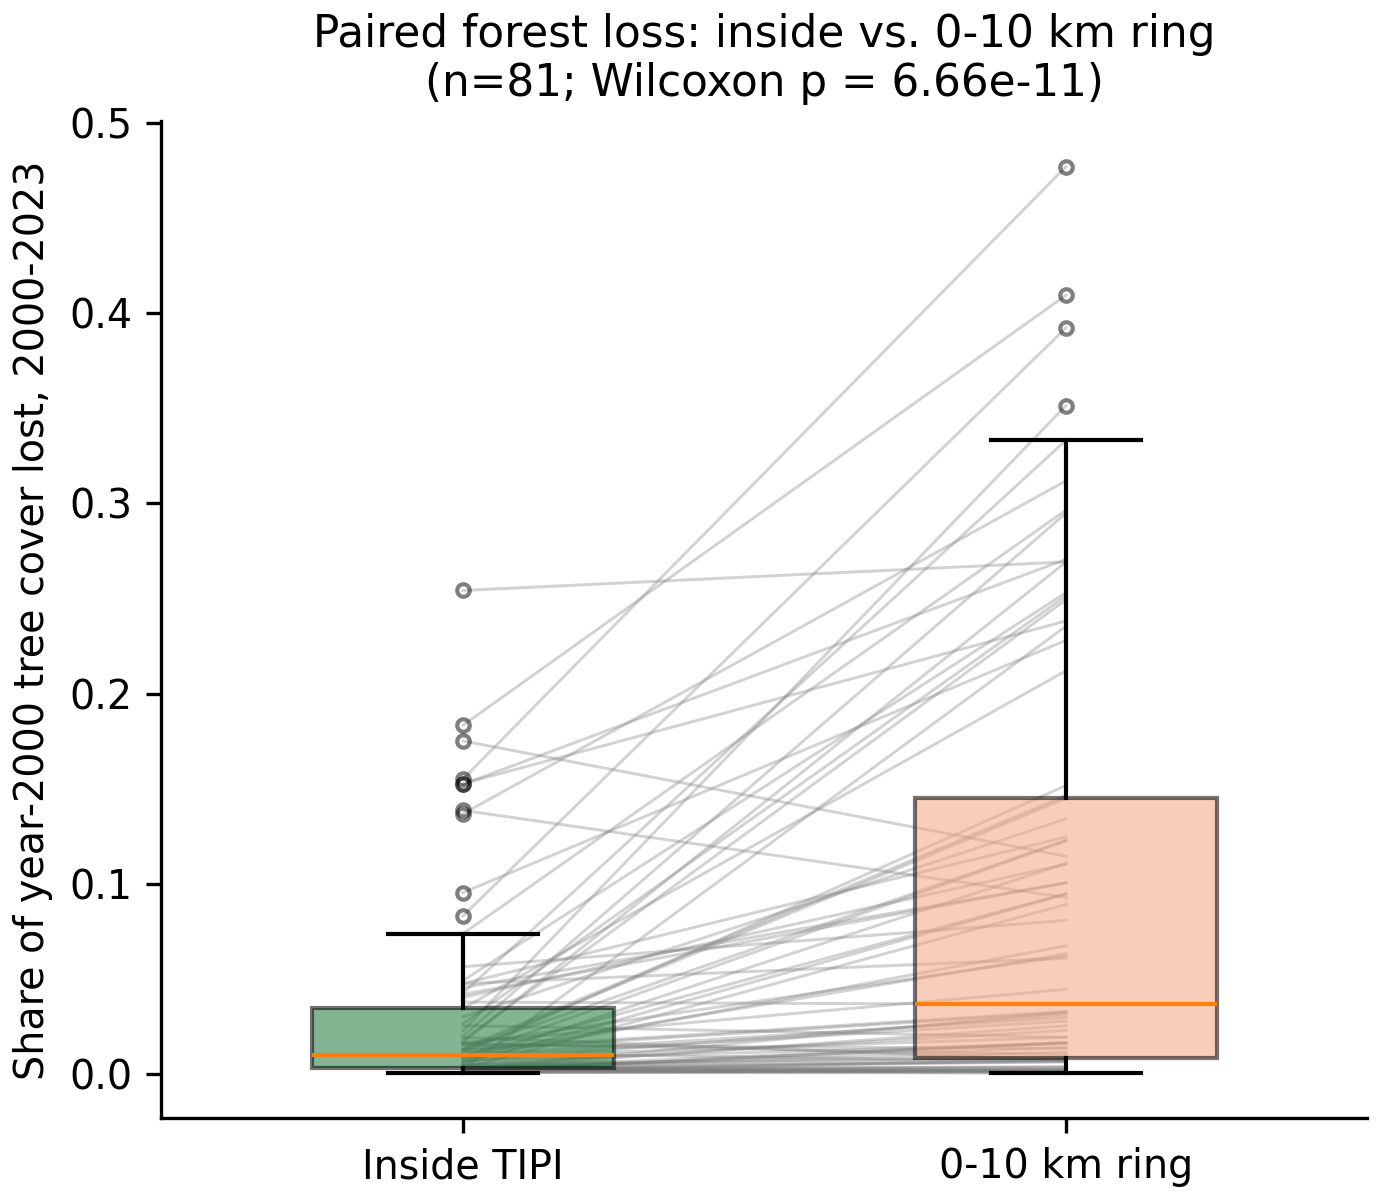
\includegraphics[width=0.62\columnwidth]{figures/fig2_paired_zones.png}
\caption{Paired forest-loss shares (fraction of year-2000 tree cover lost 2000--2023) inside \tipi{} versus their 0--10\,km rings. Grey lines connect paired values for each of the $n=81$ territories.}
\label{fig:paired}
\end{figure}

\begin{figure}[t]
\centering
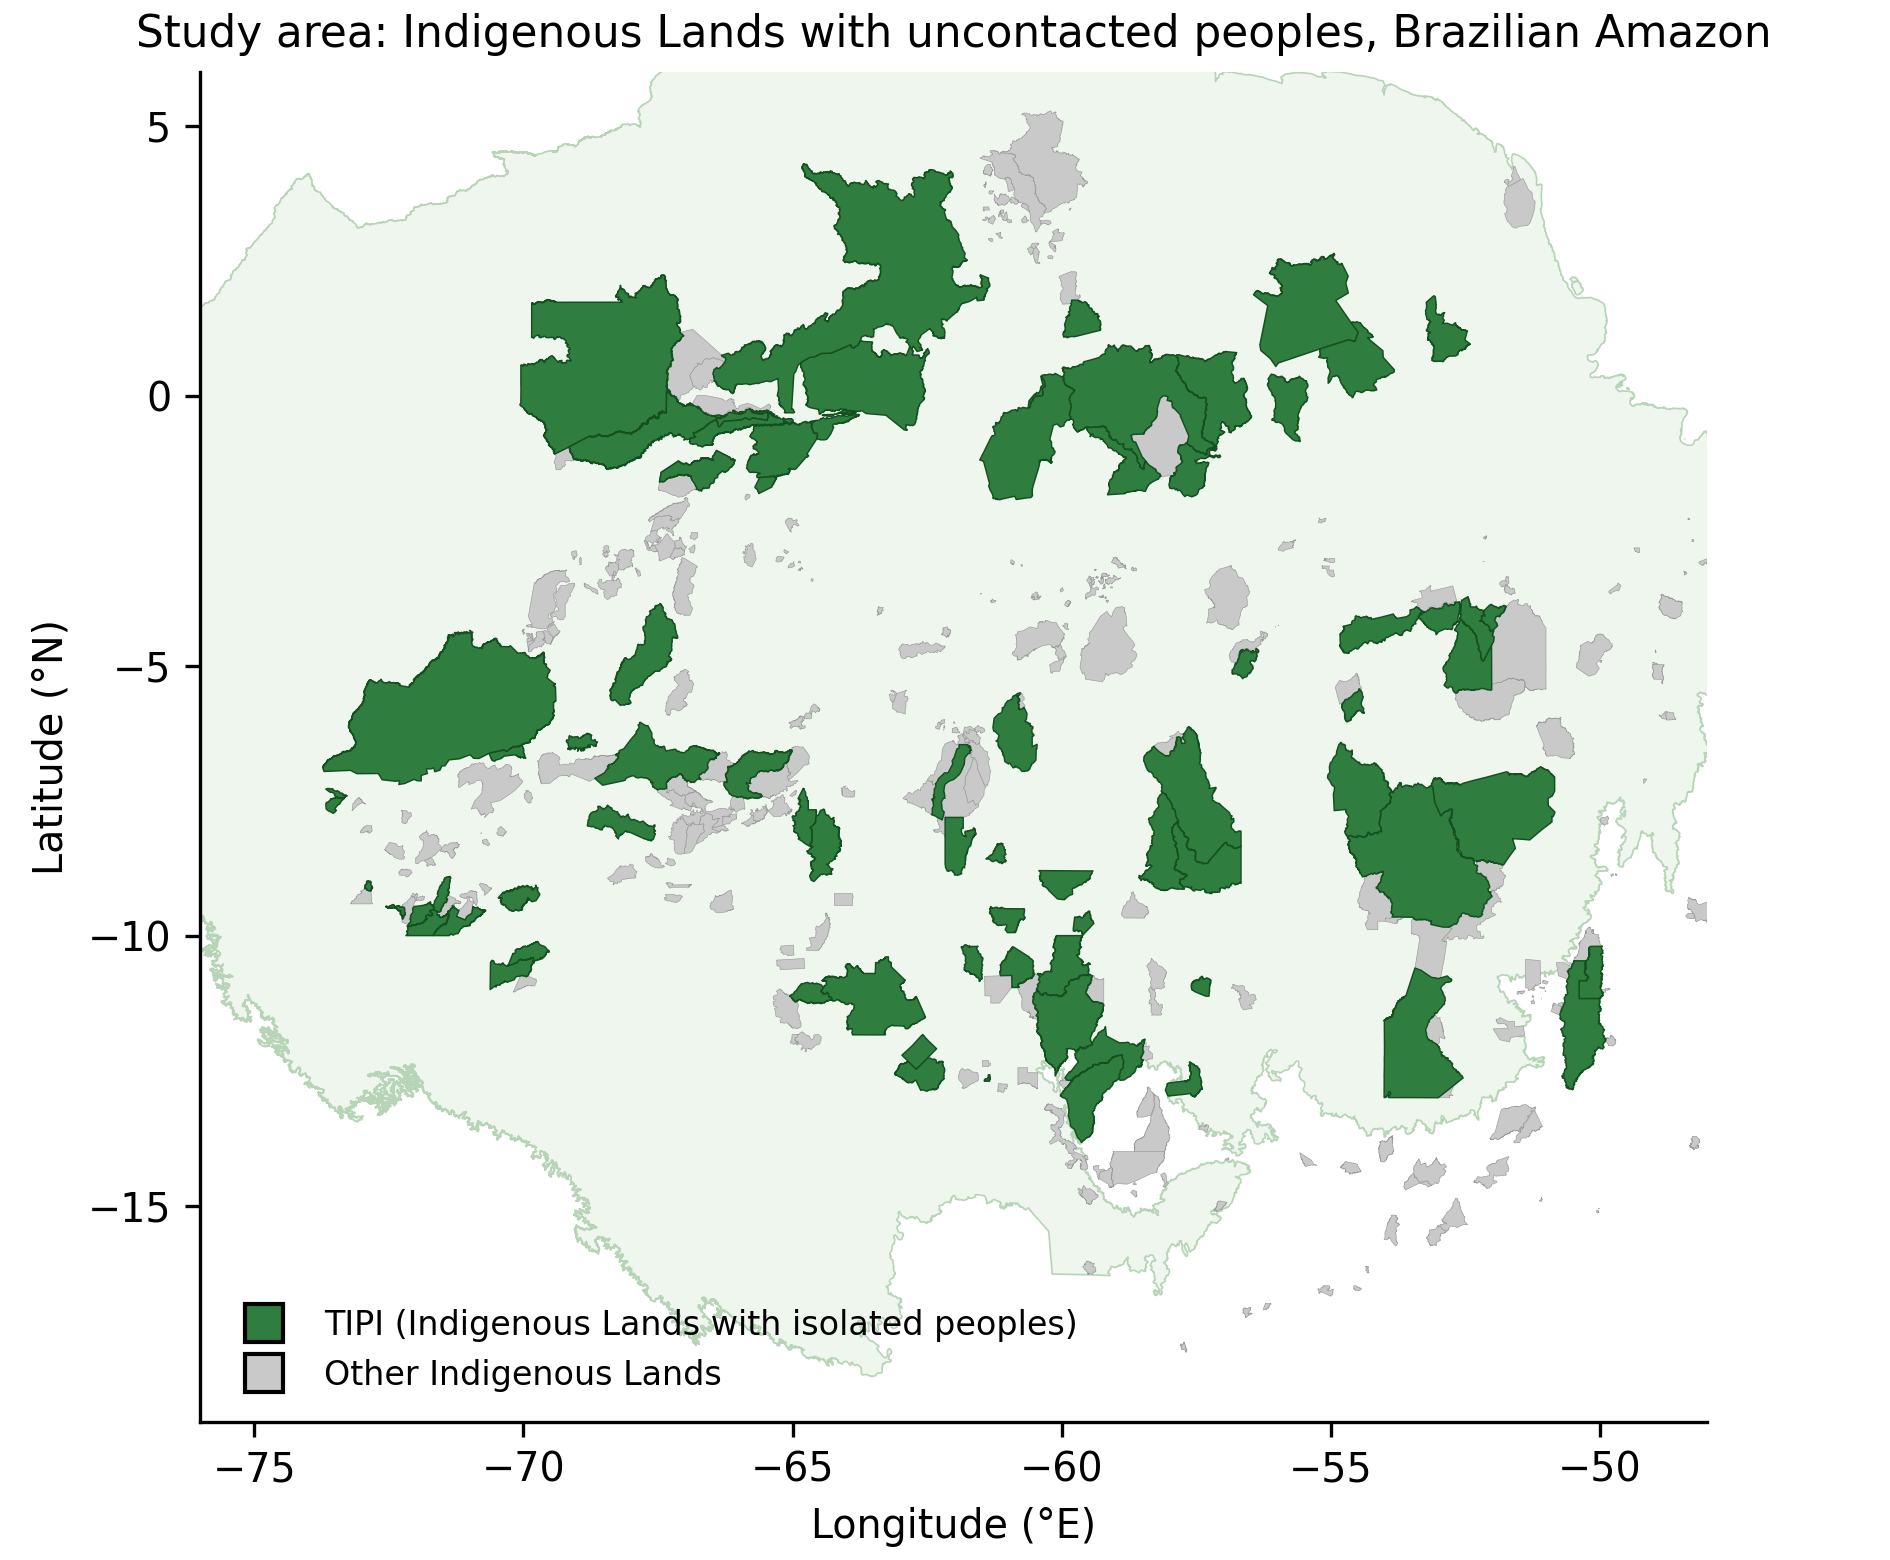
\includegraphics[width=0.8\columnwidth]{figures/fig1_study_area.png}
\caption{Study area. Green polygons are the 81 Indigenous Lands with isolated-peoples presence (\tipi{}); grey polygons are other official FUNAI Indigenous Lands within the analysis extent. Map coordinates are approximate; no settlement or record locations are shown.}
\label{fig:area}
\end{figure}

\subsection{Annual trajectories}
Inside loss was negligible and stable through 2015 (below 0.08\% of tree cover per year), then rose sharply in 2016 (0.41\%) --- a year combining a severe drought-fire season with national environmental-governance deterioration --- and remained elevated through 2023 (0.06--0.18\% per year). Aggregate inside loss more than tripled between the decades: 3.75 million loss pixels in 2001--2010, 10.5 million in 2011--2018, and 5.9 million in the five years 2019--2023. Ring trajectories mirror the same 2016--2017 peak (up to 0.73\% per year in the 10--50\,km ring), indicating that the pressure regime around these territories intensified across the board rather than only at their edges (Figure~\ref{fig:annual}).

\begin{figure}[t]
\centering
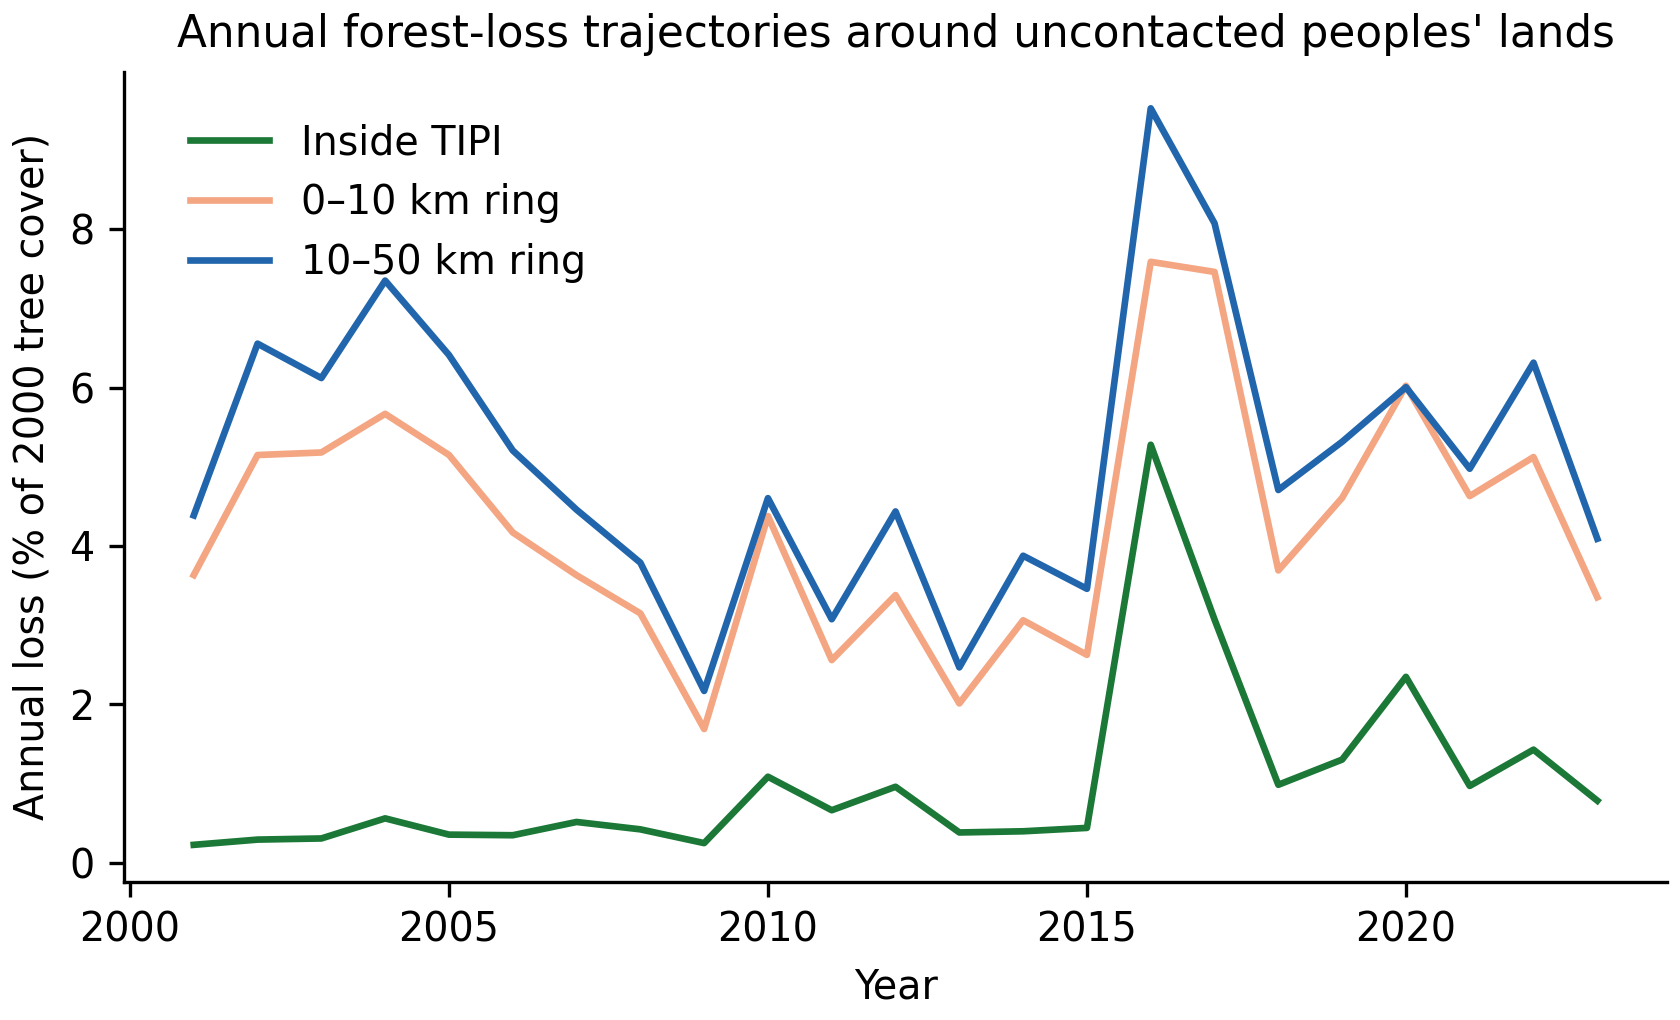
\includegraphics[width=0.85\columnwidth]{figures/fig3_annual_curves.png}
\caption{Annual forest loss as a percentage of year-2000 tree cover, aggregated across the 81 \tipi{} for each zone.}
\label{fig:annual}
\end{figure}

\subsection{RQ2: accessibility (H2)}\label{sec:access}
Ring-level pressure around \tipi{} is strongly associated with distance to the nearest city ($\rho=-0.457$, $p=1.81\times10^{-5}$; Holm-adjusted $p=5.43\times10^{-5}$; Figure~\ref{fig:access}). Conversely, distance to linear pipeline and utility corridors shows no significant correlation with ring pressure ($\rho=-0.158$, $p=0.159$; adjusted $p=0.159$). This contrast is revealing: diffuse settlement frontiers, logging access roads, and riverine trading posts centered on municipal urban hubs drive the active clearing of buffer rings, whereas isolated utility rights-of-way do not independently structure landscape deforestation.

\begin{figure}[t]
\centering
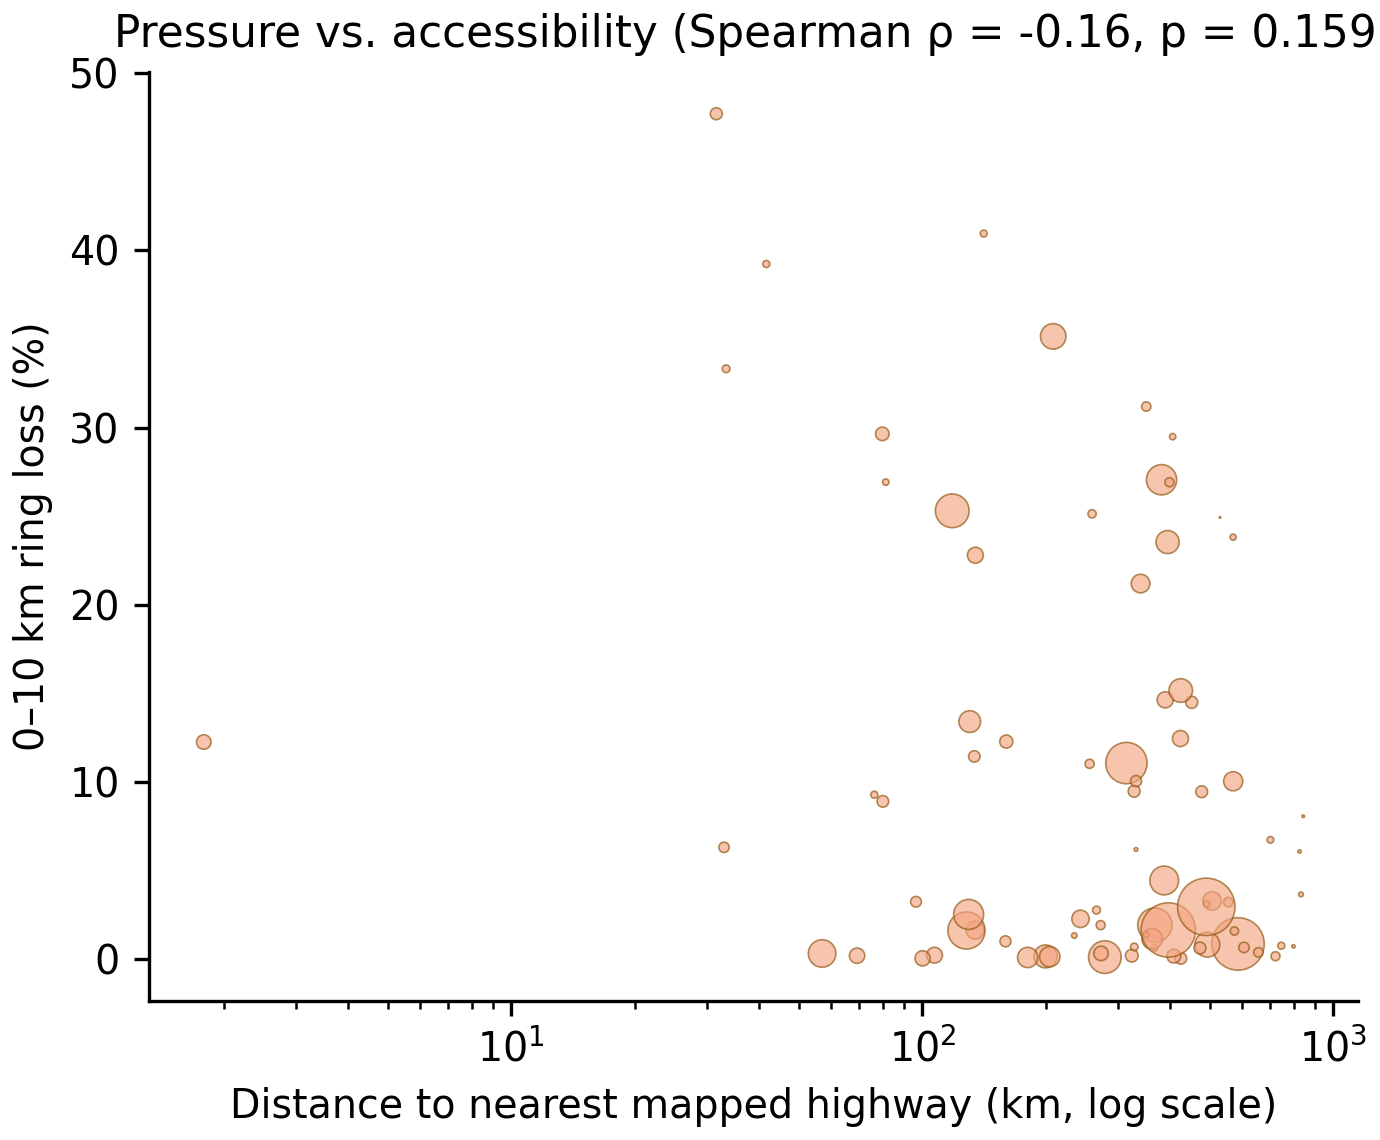
\includegraphics[width=0.62\columnwidth]{figures/fig5_accessibility.png}
\caption{0--10\,km ring loss share versus distance to the nearest mapped utility corridor (log scale); point area proportional to territory size.}
\label{fig:access}
\end{figure}

\subsection{RQ3: concentration and hotspots (H3)}
Pressure is highly concentrated. The Gini coefficient of absolute 0--10\,km ring loss across the 81 \tipi{} is 0.631 (Gini of loss share: 0.607); the top quintile of territories holds 63.5\% of aggregate ring loss, and the ten highest-pressure territories alone account for 48.5\% (Table~\ref{tab:top10}).

Examining these top-pressure territories reveals the profound buffering power of demarcation under extreme external threat (Table~\ref{tab:top10}). Uru-Eu-Wau-Wau (Rond\^onia) experienced the highest absolute external destruction, losing 222{,}349\,ha in its immediate 0--10\,km buffer ring (35.15\% of the ring's tree cover), yet deforestation inside the territory was restricted to 2.27\% (41{,}654\,ha out of 1.83 million hectares). Even more dramatically, Ba\'u (Par\'a) was besieged by 153{,}702\,ha of external clearing in its ring (23.54\% ring loss share), but suffered merely 0.25\% forest loss internally (3{,}808\,ha). In territories undergoing severe illegal invasion fronts, such as Arariboia in Maranh\~ao (15.50\% inside loss vs.\ 47.71\% in its ring) and Parque do Xingu in Mato Grosso (15.23\% inside loss vs.\ 27.06\% ring loss), internal clearing, while deeply alarming for isolated inhabitants, remained substantially lower than the near-total conversion of surrounding lands. Flagship uncontacted reserves such as Massaco (1.25\% inside loss) and Rio Omer\^e (0.59\% inside loss, surrounded by a 26.6\% ring) demonstrate that dedicated protection can halt clearing even in critical agricultural frontiers.

\begin{table}[htbp]
\centering
\caption{Ten highest-pressure \tipi{} ranked by absolute forest loss in the surrounding 0--10\,km ring, 2000--2023.}
\label{tab:top10}
\small
\begin{tabular*}{\columnwidth}{@{\extracolsep{\fill}} l l r r r r}
\toprule
Territory & State & Official Area (M ha) & 0--10\,km Ring Loss (ha) & Ring Loss Share (\%) & Inside Loss Share (\%) \\
\midrule
Uru-Eu-Wau-Wau & RO & 1.87 & 222{,}349 & 35.15 & 2.27 \\
Parque do Xingu & MT, PA & 2.64 & 201{,}849 & 27.06 & 15.23 \\
Kayap\'o & PA & 3.28 & 184{,}581 & 25.31 & 4.91 \\
Ba\'u & PA & 1.54 & 153{,}702 & 23.54 & 0.25 \\
Menkragnoti & PA, MT & 4.91 & 123{,}626 & 11.08 & 0.64 \\
Arariboia & MA & 0.41 & 112{,}000 & 47.71 & 15.50 \\
Cachoeira Seca & PA & 0.73 & 108{,}125 & 22.84 & 9.54 \\
Nambikwara & MT & 1.01 & 105{,}702 & 21.21 & 3.45 \\
Parque do Aripuan\~a & MT, RO & 1.60 & 101{,}597 & 15.17 & 1.08 \\
Yanomami & RR, AM & 9.66 & 83{,}290 & 3.01 & 1.01 \\
\bottomrule
\end{tabular*}


\end{table}

\begin{figure}[t]
\centering
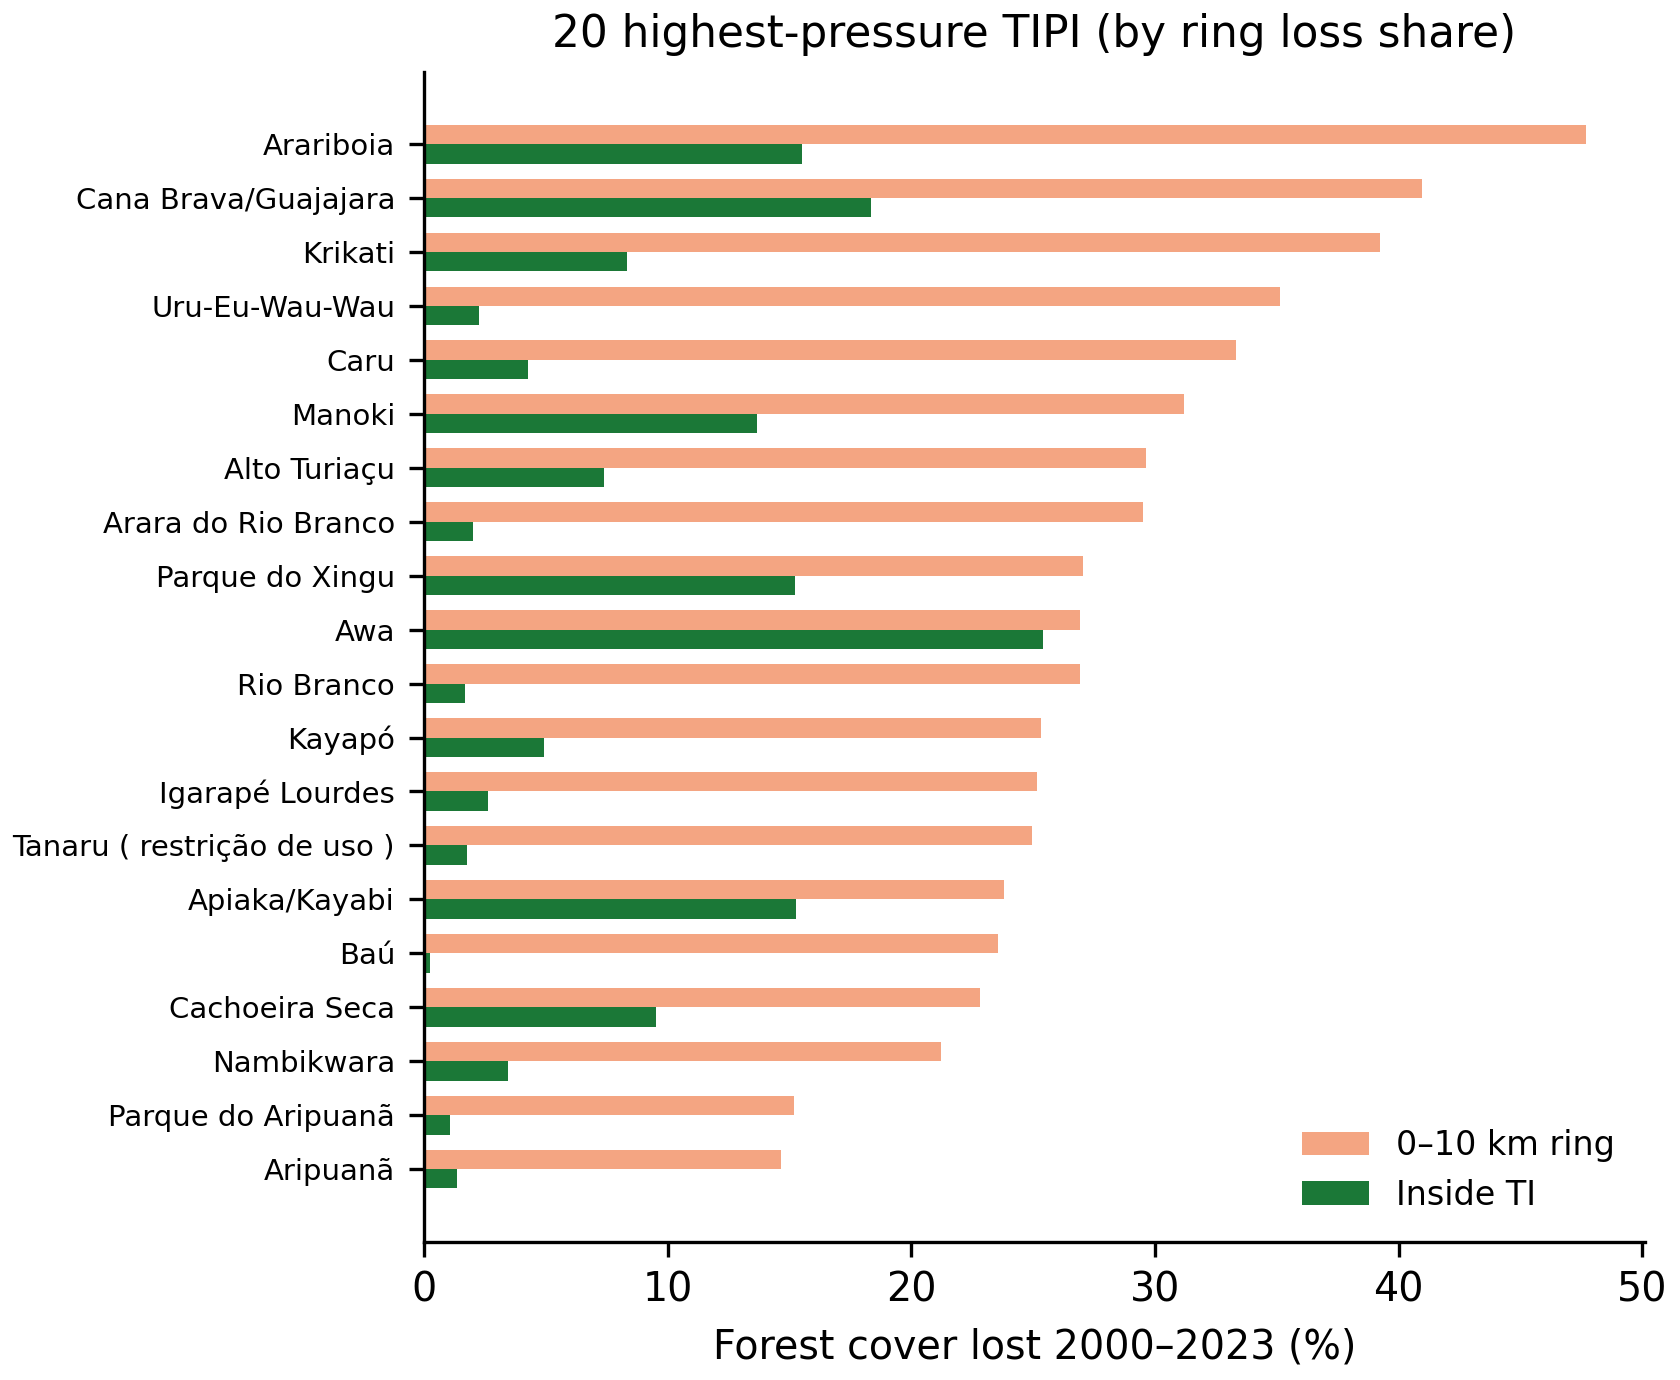
\includegraphics[width=0.8\columnwidth]{figures/fig4_top_pressure.png}
\caption{Twenty highest-pressure \tipi{} ranked by 0--10\,km ring loss share (sand), with inside loss share (green) overlaid.}
\label{fig:top}
\end{figure}

\section{Discussion}\label{sec:discussion}

\subsection{Interpretation}
Three findings stand out. First, the lands of uncontacted peoples are, quantitatively, the best-buffered Indigenous Lands in the Brazilian Amazon: 1.01\% median internal loss over 24 years, 3.6 times below their immediate surrounding rings, 5.3 times below their wider landscape buffers, and 2.5 times below matched non-isolated controls. Given that these territories host the only human populations for whom forest loss translates directly into existential risk, this asymmetry demonstrates the monumental protective success of formal demarcation and autonomous Indigenous monitoring.

Second, this buffer is under intense and concentrated pressure. External deforestation is not evenly dispersed; nearly half of all surrounding loss is concentrated around just ten territories in the soy and cattle frontiers of Rond\^onia, Par\'a, Mato Grosso, and Maranh\~ao. 

Third, the finding that municipal city distance ($\rho = -0.457$) strongly correlates with external pressure confirms that deforestation expands along diffuse agricultural and settlement frontiers. Where formal territorial protection is weakened by staffing deficits --- as documented by FUNAI's 2024 audit noting 74 vacant field posts and 12 unprotected records --- external buffer loss directly threatens the territorial integrity of uncontacted groups.


\section{Ethical Considerations}\label{sec:ethics}

This study was designed around a binding constraint: uncontacted peoples cannot consent to be studied, and any approach --- physical or informational --- that increases contact risk is unacceptable. Brazil's no-contact policy (in force since 1987), ILO Convention 169, and UNDRIP frame isolation as a choice that outsiders must respect \citep{pringle2014,ilo169,undrip}. Accordingly:

\begin{enumerate}[leftmargin=1.4em, itemsep=1pt]
\item \textbf{No contact.} The study uses exclusively remote, public, aggregate data. No field work, overflights, interviews, or interactions of any kind are proposed or implied.
\item \textbf{No location disclosure.} Coordinates of isolated-peoples records and occupation areas are used only internally to link records to official territory boundaries. No figure, table, or repository artefact publishes settlement or record locations; all outputs are aggregated to Indigenous-Land boundaries (public policy artefacts) or to regional summaries.
\item \textbf{Respectful framing.} We describe peoples, not ``tribes'', and make no claims about lifeways; the object of measurement is land and threat, not people.
\item \textbf{Data protection.} The raw record layer is excluded from the repository by default.
\end{enumerate}

\section{Conclusions and Future Research}\label{sec:conclusion}

Using only open data, we provide the first territory-level quantitative assessment of forest-loss pressure on Brazil's Indigenous Lands hosting uncontacted peoples. Between 2000 and 2023 these 81 lands lost 1.01\% of their year-2000 tree cover internally --- 3.6 times less than their immediate surroundings, 5.3 times less than wider regional buffers, and 2.5 times less than matched non-isolated Indigenous Lands --- confirming their exceptional buffering role. But this buffer is under concentrated assault: internal loss tripled after 2011, pressure concentrates sharply (top quintile: 63.5\% of aggregate ring loss) in documented crisis sites, and the state's protection apparatus was audited in 2024 as under-staffed and leaving twelve records wholly unprotected.

Future work should pursue four directions: (i) causal designs exploiting restriction-of-use ordinances and demarcation timing (staggered difference-in-differences over the territory panel) to separate protection from remoteness; (ii) extension to Peru, Colombia, and Ecuador via RAISG's isolated-peoples layers, testing external validity beyond Brazil; (iii) integration of fire and degradation products (active-fire archives, canopy-height change) to capture sub-canopy pressure invisible to gross-clearing products; and (iv) a systematic, ethics-preserving assessment of the \emph{protection-coverage gap} --- records without any territorial instrument --- by joining the audited record registry to protection-layer geometry.

\section*{Declarations}
\textbf{Funding.} None. \textbf{Conflicts of interest.} None declared. \textbf{Data and code availability.} All data are public (Table~\ref{tab:data}); all code, configuration, result files, and the audit trail are available in the open repository accompanying this preprint. \textbf{AI-assistance disclosure.} AI tools were used for code development and manuscript drafting under the author's direction; the author verified all results, retains full responsibility for the work, and discloses this assistance in line with venue policy. \textbf{Ethics.} No human subjects, no animals, no field work; see Section~\ref{sec:ethics}.



\bibliography{references}

\end{document}

